\documentclass[12pt]{article}
\usepackage[brazil]{babel}
\usepackage[utf8]{inputenc}
\usepackage{lingmacros}
\usepackage{tree-dvips}
\usepackage{graphicx}
\usepackage{authblk}
\usepackage{url}

\title{Colorações próprias: um estudo aprofundado}
\author{Autores: Gabriel Souza, Jonathan Melo}
\affil{Orientador: Prof. Celso A. Weffort-Santos }
% \date{06 de Abril, 2020}

\begin{document}
	
	\maketitle
	
	\section{Introdução}
	Nesta seção serão mostrados os conceitos iniciais sobre grafos, os objetivos procurados durante a pesquisa sobre o tema, a justificativa para o tema escolhido, bem como a notação que será usada durante o documento para a descrição dos conceitos.Para os demais conceitos e notações não definidos neste documento, indicamos ao leitor o livro ``Graph Theory'' de J. Bondy e U. S. R. Murty~\cite{BondyM08}
	
	A ideia inicial do que hoje se tornou um dos grandes estudos da área da matemática e tecnologia partiu de Leonhard Euler (1707 –1783) matemático e físico suíço que teve sua motivação para a criação do problema das Sete Pontes de Königsberg.
	
	A cidade de Königsberg (após 1946 chamada de Kaliningrado) é uma cidade russa onde em uma parte do seu território existe um rio que separa a cidade em duas áreas. No decorrer desse rio existiam 7 pontes conectando as duas áreas da cidade formando algo parecido com a imagem que podemos ver na Figura 1.
	
	\begin{figure}[!htb]
		\centering
		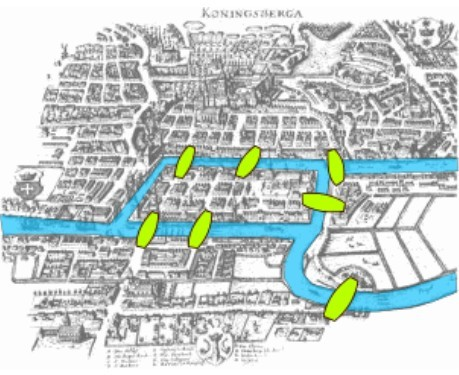
\includegraphics[width=8cm, height=8cm]{pontesKonisberg}
		\caption{Mapa das pontes de Königsberg}    
	\end{figure}
	
	A motivação de Euler veio a partir de uma discussão feita pelos moradores da cidade, os mesmos argumentavam se era ou não possível atravessar todas as pontes sem repetir nenhuma delas durante o trajeto.
	
	Euler provou que era impossível este trajeto e deu início ao primeiro teorema da Teoria de Grafos, antes de introduzirmos os termos técnicos, se fossemos trazer este teorema para o problema das pontes, Euler provou que para que esse caminho fosse possível, cada uma das regiões do mapa precisaria ter um número par de pontes incidentes a ele. O teorema descrito, levou o nome de Ciclo Euleriano.
	
	Após criado o conceito inicial sobre grafos, um outro matemático introduziu uma nova forma de desenharmos um grafo, William Thomas Tutte (1917-2002) definiu que um grafo poderia ser representado por vértices(pontos) e arestas(linhas), aonde os vértices são interligados por arestas conectados a eles, trazendo esta definição para o problema das sete pontes, definiríamos que ponte do mapa seria uma aresta e cada ilha seria um vértice, tendo sua definição visual parecida com a Figura 2.
	
	
   \begin{figure}[!htb]
		\centering
		\includegraphics[width=6cm, height=6cm]{grafoKönigsberg}
		\caption{ Grafo das sete pontes de Königsberg}    
	\end{figure}


	\subsection{Conceitos técnicos da Teoria de Grafos}
    Como vimos na seção anterior, após as descobertas de Euler, foram introduzidos novas maneiras de lidarmos com problemas parecidos.
	Um grafo $G$ é composto por vértices $v$ e arestas $e$ sendo sua composição completa denotada como $G (v, e)$. O número de vértices contidas em um grafo é definido como a Ordem do grafo $n$ e o número de arestas é o seu Tamanho $m$. Esses conceitos iniciais sobre o tema, podem ser desdobrados em outros conceitos que complementam e inserem novas definições para o grafo.
	
	\subsubsection{Vizinhança de vértices}
	
	Em um grafo $G$ existem os vértices $u$ e $v$ ligados por uma aresta de $G$, baseado nessas afirmações podemos definir que os vértices $u$ e $v$ são adjacentes ou vizinhos, caso em nosso grafo existissem mais duas vértices ligadas a vértice $v$ sendo elas $z$ e $w$, poderíamos a partir disso definir que a vizinhança de $V$ é: $n (V) \{u, z, w\}$, representado visualmente na Figura 3. 
		
	\begin{figure}[!htb]
		\centering
		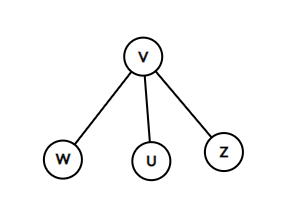
\includegraphics[width=5cm, height=5cm]{vizinhanca}
		\caption{Representação visual da vizinhança de $v$}    
	\end{figure}
	
	
	\subsubsection{Grau de vértices}
	Em um grafo $G$ contendo os vértices $V = \{u, x, w\}$ e as seguintes vizinhanças de vértices $n(u) = \{x, w\}$, $N(x) = \{u\}$ e $N(w) = \{u\}$.	
	Definimos que o grau de um vértice é o número de arestas incidentes nele e é denotado como $d(v)$, baseado nessa condições e utilizando o exemplo criado, denotaríamos o grau de $u$ como $d(u) = 2$, $d(x) = 1$ e $d(w) = 1$, visto que baseado em nossa vizinhança esse é o número de arestas incidentes em cada um de nossos vértices.
	
	\subsection{ Coloração própria de vértices em grafos}
	Sendo esse o tema escolhido para as nossas pesquisas, a definição do problema diz que para termos uma coloração própria dentro de um grafo, vértices que são adjacentes não podem ter a mesma cor. Desta maneira podemos definir também um número cromático para o nosso grafo denotado de $\chi(G)$, número esse que é definido como o menor número de cores possíveis para pintar um grafo de forma que cumpramos todas as regras definidas para um grafo com coloração própria.
	Um grafo $G$ é considerado k-Colorivel, se pudermos dentro dele usar um número $k$ de cores para sua coloração sem que afetemos a regra da coloração própria.
	
	\subsubsection{História e o problema das quatro cores}
	
	Antes de introduzirmos a motivação para o problema da coloração própria, é preciso definir o conceito de um grafo planar, visto que este tipo de grafo foi a motivação inicial para a criação da primeira definição da coloração própria de grafo.
	Um grafo $G$ é considerado planar se puder ser desenhado no plano sem que nenhuma de suas arestas se cruzem, exemplo de um grafo planar existente na Figura 4.
		
	
	A primeira ideia de coloração própria se deu em 1852 aonde o matemático Francis Guthrie criou a teoria que para todo mapa o número mínimo de cores necessárias para pinta-lo para que nenhuma de suas regiões que partilhassem fronteiras fossem pintadas da mesma cor era sempre quatro~\cite{FourColorTheorem}.
	
	
	Em 1879 Alfred Bray Kempe publicou a primeira suposta solução para a teoria das quatro cores em um trecho do livro intitulado de ''On the geographical problem of the four colors''\cite{OnGeographical} , solução essa que foi considerada incorreta por Percy Heawood em 1890, que também foi o criador do teorema das Cinco cores, e provou a veracidade do mesmo em seu livro publicado em 1890 chamado de ``Map colour theorem ''~\cite{MapColor}.
		
	\begin{figure}[!htb]
		\centering
		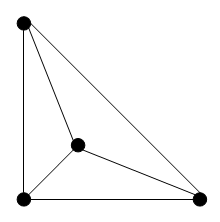
\includegraphics[width=3cm, height=3cm]{grafoPlanar}
		\caption{Grafo planar}    
	\end{figure}

	Apesar de ser considerado incorreta a teoria de Kempe, ela foi grande influenciadora para que em 1977 Kenneth Appel (1932-2013) e Wolfgang Haken(1928) com o auxílio do uso de um computador, provassem novamente que a teoria das quatro cores era correta.As informações desses resultados podem ser encontradas nos artigos ``Every planar map is four colorable. Part I. Discharging, \cite{EveryFourPart1} '' e 	``Every planar map is four colorable. Part II. Reducibility, \cite{EveryFourPart2} ''
	
	
	Os mapas estudados por esses matemáticos são considerados mapas que podem ser representados por um grafo, o nome que esse grafo leva é grafo dual. 
	
	\begin{figure}[!htb]
		\centering
		 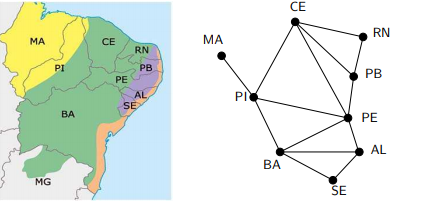
\includegraphics[width=8cm,height=4cm]{grafoDual}
		\caption{Grafo Dual}    
	\end{figure}

	
	\subsubsection{Complexidade da solução}
	
	Nos problemas envolvendo coloração própria de vértices, encontrar um número $k$ de cores possíveis é mais simples do que encontrar $\chi(G)$, visto que se tivermos $n$ vértices podemos ter que $k = n$ e ter uma cor para cada vértice do grafo. Baseado nessa afirmação podemos concluir que a maior dificuldade para este tema é encontrar o número cromático da instância ou o menor número de cores possível, transformando este tema em um problema computacional extremamente difícil aonde validar uma solução é simples porém achar uma solução se torna muito difícil.
	Validar uma solução como citado acima nos casos de coloração própria é simples pois baseado na instância que nos foi dada, podemos validar todos os vértices adjacentes a ele de forma rápida, validando se eles tem ou não a mesma cor. Já para criarmos uma solução isso se torna extremamente difícil, dado um grafo $G$ aonde $V(G) = \{v_{1}, .... V_{n} \}$, para encontrar a solução com o melhor número cromático desta instância devemos validar todas as situações e adjacências de todos os vértices do grafo, para isso normalmente são utilizados algoritmos de busca que serão citados e explicados posteriormente.
	z
	\subsubsection{Aplicação reais do tema}
	
	Neste tópico iremos descrever algumas aplicações no nosso dia aonde o auxílio do conceito de coloração própria de grafos seria útil para encontrarmos a melhor solução para o problema escolhido. Os Exemplos citados foram adaptados do autor Atílio Gomes Luiz em sua apresentação sobre coloração de grafos intitulada de  ''Coloração de grafos e suas aplicações~\cite{ColoracaoEAplicacoes}''.

	
	\begin{itemize}
		
	
    \item \textbf{Organização de provas de uma universidade.}	Um dos melhores de exemplo do uso da coloração própria em aplicações reais é na organização de provas de uma universidade aonde é necessário que duas disciplinas que contiverem alunos em comum não podem ter suas provas agendadas no mesmo horário, levando-nos a seguinte pergunta, qual seria o menor número de horários que a universidade teria de usar para aplicar todas as provas respeitando as regras da instância?
	
    \item \textbf{Organizações de produtos químicos em uma indústria.} Em uma indústria química existem $n$ produtos, aonde muitos deles compartilham o mesmo tipo de composição, produtos esses que não podem ser colocados juntos devido a possibilidade de que uma reação química estragassem os mesmos. Baseado nessa instância, qual seria o menor número de compartimentos possíveis para guardar esses produtos de forma que produtos com a mesma composição não podem ser colocados juntos. Para organizar a possível coloração própria dessa situação e definir o seu grafo, primeiro teríamos que abstrair as informações dadas e transforma-las para a estrutura de um grafo. Nesse caso iriamos definir que cada composto iria ser um vértice e compostos que colocados juntos poderiam executar uma reação química estariam ligados por uma aresta, baseado nisso poderíamos descobrir qual seria o menor numero de cores usadas para colorir o grafo e voltando para o nosso problema inicial poderíamos descobrir o menor numero de compartimentos possíveis para guarda esses produtos.
   \end{itemize}
	\subsubsection{Algoritmos de coloração conhecidos}
	
	Nesta seção iremos mostrar conceitos de algoritmos conhecidos que auxiliam na obtenção da melhor solução para uma instância de coloração própria, visto que a complexidade deste problema é extremamente difícil, a maioria de seus algoritmos são baseados na premissa da busca incansável, aonde iremos executar todas as situações da instância a fim de no final separar a melhor delas.
	
   \begin{itemize}
		
   \item \textbf{Força bruta.}	Dado um grafo $G$ simples onde $V(G) = \{v_{1}, ... V_{N},\}$ o algoritmo de força bruta com o objetivo de buscar um k-coloração iria verificar cada uma das Kn atribuições possíveis verificando se cada uma delas está correta. Em uma instância pequena do problema, o algoritmo de força bruta encontraria o resultado de forma relativamente rápida, porém se consideramos que quanto maior a instância do problema maior seria a quantidade de atribuições que deverão ser testadas, esse algoritmo se torna inutilizável e computacionalmente inviável.
	
	
    \item \textbf{Algoritmo guloso.} O algoritmo guloso é aquele que faz sempre a melhor escolha local minimizada, esperando que essa escolha se torne também a melhor escolha em um estado global da instância do problema.
	Este algoritmo sempre irá trazer a solução para o problema, porém esta solução não necessariamente é a melhor possível, e sim a melhor que o algoritmo encontrou dado as suas condições de busca.
	
	
    
	\item \textbf{Algoritmo de Welsh-Powell.} Como citado no livro "Algoritmos e heurísticas - Desenvolvimento e avaliação de performance" escrito por Ruy Eduardo Campello e Nelson Maculan~\cite{AlgortimosHeuristicas}  o algoritmo de Welsh-Powell foi criado em 1976 e é um algoritmo guloso que visa a obtenção inicial do grau de cada vértice do grafo e ordenação dos mesmos em ordem decrescente do seu grau. Com base nisso sabemos que dado essa ordenação será associado uma cor para o primeiro vértice da lista de vértices ordenados, e também aos próximos vértices da lista que não são adjacentes aos vértices já coloridos com a primeira cor selecionada. Será feito este mesmo processo para os próximos vértices que ainda não foram coloridos, porém agora usando a próxima cor.
	
   \end{itemize}
 
	\subsection{Objetivos}
	
	O tema dessa pesquisa é muito amplo e completo, de forma que seus conhecimentos se desdobram em várias áreas da ciência da computação e matemática. O objetivo deste projeto é o estudo teórico de várias técnicas e conceitos presentes na literatura. Ademais, deseja-se o avanço científico do estudo do tema, propondo novos resultados em colorações de grafos, seja em algoritmos ou em propriedades estruturais. Alguns objetivos pontuais são descritos em seguida.
	
	\begin{enumerate}
		\item Desenvolver  o conhecimento e a desenvoltura na área da matemática discreta, com aplicações em Teoria de Grafos e, especificamente, na área de colorações próprias de grafos.
		\item Criar a capacidade de reconhecer o estado da arte, através da leitura de artigos científicos publicados em periódicos de renome, pesquisando a literatura vigente e identificando problemas em aberto no tópico.
		\item Conhecer e estudar os principais resultados teóricos na área de colorações de grafos, como, por exemplo, o Teorema das Quatro Cores, a equivalência de bipartição, o Teorema de Brooks~\cite{Brooks41}, entre outros.
	\end{enumerate}
	
	
        \section{Material e métodos}

       No desenvolvimento desse projeto, serão necessários um ambiente para estudo e para as reuniões com o orientador, e acesso às bibliotecas física e digital, para possíveis consultas.

       Os estudos serão realizados em dupla, com o auxílio do orientador durante nossas reuniões semanais para   alinhamentos do projeto e para sanar possíveis dúvidas. Toda semana, o orientador se compromete a levantar questionamentos sobre o andamento do projeto, os resultados alcançados durante a semana e as metas de pesquisa para a próxima. Por fim, ressaltamos que o projeto será desenvolvido em conjunto com a disciplina teórica J702 - Teoria de Grafos, do qual o orientador é o professor. Portanto, o projeto de pesquisa permitirá que os alunos abordem com mais profundidade os conceitos expostos em sala de aula, além de ter contato com outras áreas da Teoria da Computação.
 
      É importante informar que, em virtude do COVID-19 e de acordo com as normas impostas pelo Governo  do Estado de São Paulo e pelo Ministério da Saúde, as reuniões semanais serão realizadas utilizando plataformas online como Zoom, Google Meet e/ou Discord. 

	
	
	\bibliographystyle{unsrt}
	\bibliography{/Projects/Iniciacaocienteifica/bibliography}
	
\end{document}


